\chapter{Lecture 4: Line Integrals \& Green's Continuous Map}
\begin{theorem}
    [Parametrized Curves]
    $$ \gamma (t) = x(t) + iy(t) \quad a \leq t \leq b $$
    $\gamma [a,b] \to \mathbb{C}$ is the image of $\gamma$.
\end{theorem}

\begin{example}
    [Circle Parametrization]
    \begin{align*}
        \gamma(t) & = \cos(t) + i\sin(t) \quad 0 \leq t \leq 2\pi \\
        \gamma(t) & = e^{it} \quad 0 \leq t \leq 2\pi
    \end{align*}
    So $\gamma$ is a circle of radius 1 centered at the origin.
    \begin{figure}[H]
        \centering
        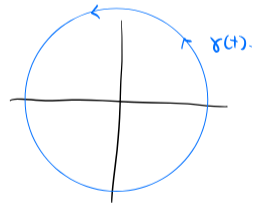
\includegraphics[width=0.5\textwidth]{LECTURE_4/circle.png}
        \caption{Circle Parametrization}

    \end{figure}
\end{example}

\begin{example}
    [Keyhole Parametrization (Section 1.6, Example 5)]
    \begin{figure}[H]
        \centering
        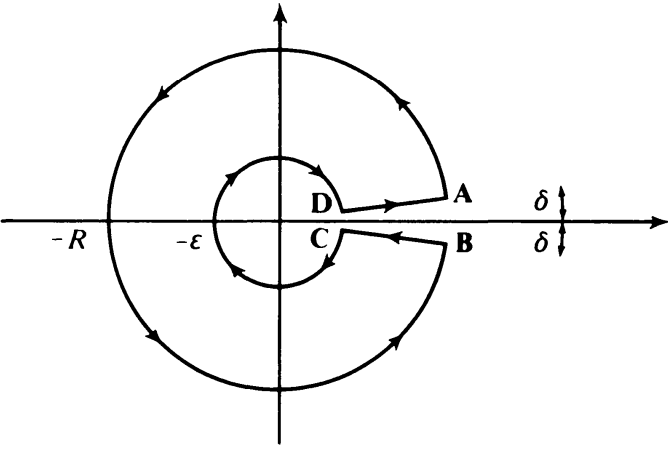
\includegraphics[width=0.5\textwidth]{LECTURE_4/parametrize.png}
        \caption{Keyhole Parametrization}
    \end{figure}
    The first part of the keyhole is parametrized by a circle of radius $R$ centered at the origin between $\delta$ and $2\pi - \delta$. This is given by the following:
    \begin{align*}
        \gamma (t) = Re^{i\theta} \quad \delta \leq \theta \leq 2 \pi - \delta
    \end{align*}
    The inner circle is parametrized by a circle of radius $\epsilon$ centered at the origin between $2\pi - \delta$ and $\delta$. Note that the direction of the parametrization is opposite to the first circle.
    The lines of the keyhole connects the two circles at $\theta = 2\pi - \delta$ and $\theta = \delta$.\\
    So the keyhole is parametrized by the following:
    \begin{align*}
        \gamma (t) = \begin{cases}
                         Re^{i\theta}          & \delta \leq \theta \leq 2\pi - \delta \\
                         te^{i(2\pi - \delta)} & R \leq t \leq \epsilon                \\
                         \epsilon e^{i\theta}  & 2\pi - \delta \leq \theta \leq \delta \\
                         te^{i\delta}          & \epsilon \leq t \leq R
                     \end{cases}
    \end{align*}
    \label{ex:keyhole}
\end{example}



\begin{definition}
    [Simple Curve]
    A curve $\gamma$ is \textbf{simple} if $\gamma(t_1) = \gamma(t_2) \implies t_1 = t_2$ for $t_1, t_2 \neq a, b$.
\end{definition}
\begin{definition}
    [Closed Curve]
    A curve $\gamma$ is \textbf{closed} if $\gamma(a) = \gamma(b)$. So if the end point meets the starting point.
\end{definition}

\begin{remark}
    We can \textit{ignore} the parametrization and talk about the curve $$Image(\gamma) \subset \mathbb{C}$$ as a subset of $\mathbb{C}$.
\end{remark}

\begin{definition}
    [$C^1$/Smooth Curve]
    A parametrized curve is $C^1$ if $\gamma'(t)$ if
    $$\gamma '(t) = x'(t) + iy'(t)$$ exists $\forall t \in [a,b]$ and is continuous.
\end{definition}

\begin{remark}
    Here, $\gamma'(a) = x'(a) + iy'(a), \gamma'(b) = x'(b) + iy'(b)$ are the 1-sided derivatives (i.e. they consider the rate of change from the left/right where the function is defined).
\end{remark}

\begin{definition}
    [Piecewise $C^1$/Smooth Curve]
    $$\text{if } \exists a = t_0 < t_1 < \ldots < t_n = b \text{ such that } \gamma |_{[t_i, t_{i+1}]} \text{ is } C^1$$
\end{definition}
\begin{figure}[H]
    \centering
    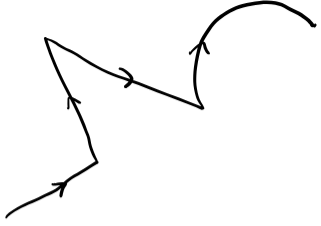
\includegraphics[width=0.5\textwidth]{LECTURE_4/piecewise-c1.png}
    \caption{Piecewise $C^1$ Curve}
\end{figure}
\section{Line Integrals}
\begin{definition}
    [Line Integral]
    if $g = u + iv, (u,v) \in \mathbb{R}^2$ is a complex-valued function and $\gamma$ is piecewise $C^1$, then the line integral of $g$ along $\gamma$ is
    $$\int_{\gamma} g(z) dz = \sum_{i=0}^{n-1}\int_{i}^{i+1} g(\gamma(t)) \gamma'(t) dt$$
    Where
    \begin{align*}
        g(\gamma(t)) \gamma'(t) & = ux' - vy' + ivx' + iuy'                        \\
                                & = (u(\gamma(t)) + iv(\gamma(t)))(x'(t) + iy'(t)) \\
    \end{align*}
    is complex multiplication.
\end{definition}

\begin{example}
    [Line Integral Example]
    Compute the line integral of $\int_{\gamma} z^2 - 3|z| + \Im (z) dz$ where $\gamma(t) = 2e^{it}, 0 \leq t \leq \pi/2$.
    \begin{align*}
        \gamma^{\prime} (t)                     & = 2ie^{it}                                                                                                \\
        g(\gamma(t))                            & = \gamma(t)^2 - 3|\gamma(t)| + \Im(\gamma(t))                                                             \\
                                                & = 4e^{2it} - 6 + 2\sin(t)                                                                                 \\
        \int_{0}^{\pi/2}g(\gamma(t)) \gamma'(t) & = (4e^{2it} - 6 + 2\sin(t))(2ie^{it})                                                                     \\
                                                & = \int_{0}^{\pi/2} 8ie^{3it} - 12ie^{it} + 4ie^{2it}\sin(t)                                               \\
        \Rightarrow \sin(t)                     & = \frac{e^{it} - e^{-it}}{2i}                                                                             \\
                                                & = \int_{0}^{\pi/2}\left( 8ie^{3it} - 12ie^{it} + 4ie^{2it}\right)\left(\frac{e^{it} - e^{-it}}{2i}\right) \\
                                                & = \int_{0}^{\pi/2} 4e^{4it} - 6e^{2it} + 2e^{3it} - 4e^{it} + 2e^{2it} - 3e^{it} + e^{3it} - e^{it}       \\
                                                & = \left(\frac{8}{3}e^{3it} - 12e^{it} - ie^{2it} - 2t\right) |_{0}^{\pi/2}                                \\
                                                & = \frac{8}{3}e^{3i\pi/2} - 12e^{i\pi/2} - ie^{i\pi} - 2\pi - \left(\frac{8}{3} - 12 - i \right)           \\
                                                & = \frac{28}{3} - \pi - \frac{38}{3}i
    \end{align*}

\end{example}

\begin{example}
    [Line Integral Example]
    Compute the line integral of $\int_{\gamma} \cos z dz$ where $\gamma(t)$ is the line segment from $-\pi/2 + i$ to $\pi + i$.
    \begin{align*}
        \gamma(t)                                  & = -\frac{\pi}{2}  + i + t(\pi + i + \frac{\pi}{2} - i) \quad 0 \leq t \leq 1                                                                         \\
                                                   & = -\frac{\pi}{2} + i + t(\frac{3\pi}{2})                                                                                                             \\\\
        \gamma'(t)                                 & = \frac{3\pi}{2}                                                                                                                                     \\\\
        \int_{0}^{1} \cos(\gamma(t)) \gamma'(t) dt & = \int_{0}^{1} \cos(-\frac{\pi}{2} + i + t(\frac{3\pi}{2})) \frac{3\pi}{2} dt                                                                        \\
        \rightarrow \cos(x + iy)                   & = \cos(x)\cosh(y) - i\sin(x)                                                                                                                         \\
                                                   & = \int_{0}^{1} \cos(-\frac{\pi}{2} + t(\frac{3\pi}{2}))\cosh(1) - i\sinh(1)\sin(-\frac{\pi}{2} + t(\frac{3\pi}{2})) \frac{3\pi}{2} dt                \\
                                                   & = \cosh(1)\int_{0}^{1} \cos(-\frac{\pi}{2} + t(\frac{3\pi}{2}))dt - i\sinh(1)\int_{0}^{1} \sin(-\frac{\pi}{2} + t(\frac{3\pi}{2})) \frac{3\pi}{2} dt \\
                                                   & = \cosh(1) - i\sinh(1)
    \end{align*}

\end{example}

\begin{theorem}
    [Length of a Curve]
    If $\gamma$ is a piecewise $C^1$ curve, then the length of $\gamma$ is
    $$\text{Length}(\gamma) = \sum_{i = 0}^{n-1}\int_{t_i}^{t_{i + 1}} |\gamma'(t)| dt$$
    So we have
    $$ |\int_{\gamma}g |\leq \max_{z \in \gamma}|g(z)| \cdot \text{Length}(\gamma) $$
\end{theorem}

\begin{proof}
    \begin{align*}
        |\int_{\gamma}g| & = |\sum_{i=0}^{n-1}\int_{i}^{i+1} g(\gamma(t)) \gamma'(t) dt|                \\
                         & \leq \sum_{i=0}^{n-1}\int_{i}^{i+1} |g(\gamma(t)) \gamma'(t)| dt             \\
                         & \leq \sum_{i=0}^{n-1}\int_{i}^{i+1} |g(\gamma(t))| |\gamma'(t)| dt           \\
                         & \leq \max_{z \in \gamma}|g(z)|\sum_{i=0}^{n-1}\int_{i}^{i+1} |\gamma'(t)| dt \\
                         & = \max_{z \in \gamma}|g(z)| \cdot \text{Length}(\gamma)
    \end{align*}
\end{proof}


\begin{theorem}
    [Green's Theorem]
    Say $ \Omega \subset \mathbb{C} $ such that $\partial \Omega$ is a finite collection of piecewise $C^1$ closed simple curves. If $g = u + iv$ is $C^1$ on $\Omega$, and
    % $$\int_{\partial \Omega} g = \int_{\Omega} \left( \frac{\partial v}{\partial x} - \frac{\partial u}{\partial y} \right) dxdy$$
    % Where $\partial \Omega$ is the boundary of $\Omega$.

    $f = p + iq$ is differentiable in $\Omega$, then ($\Re{p, q}$ have $1^{st}$ order derivatives). Then
    $$\int_{\partial \Omega} f dz = i \int\int_{\Omega} \left( \frac{\partial f}{\partial x} - i\frac{\partial f}{\partial y} \right) dxdy$$
    Where $\partial \Omega$ is the boundary of $\Omega$.
\end{theorem}

\begin{figure}[H]
    \centering
    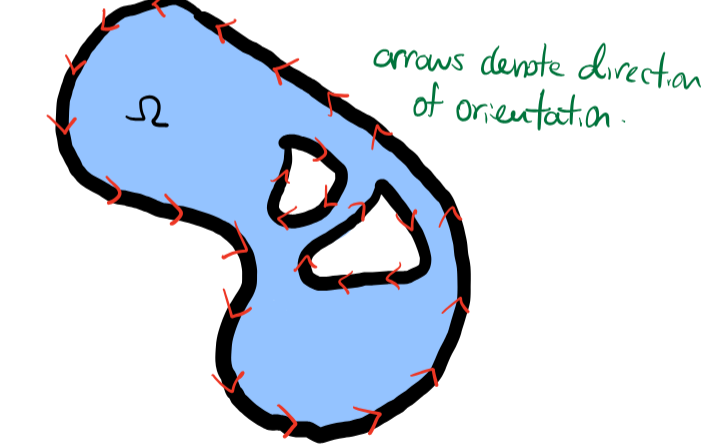
\includegraphics[width=0.5\textwidth]{LECTURE_4/green.png}
    \caption{Green's Theorem}
\end{figure}

\begin{corollary}
    Let's just show this with the real part of $f$. If $dz = dx + idy$, then
    \begin{align*}
        \Re(fdz) & = \Re((p + iq)(dx + idy)) \\
                 & = pdx - qdy               \\
    \end{align*}
    If $f$ is differentiable in $\Omega$, then the following holds (as will be shown by the Cauchy-Riemann equations next lecture). Note: This is not the derivative.
    \begin{align*}
        \Re{(i \left(\frac{\partial f}{\partial x} + \frac{i \partial f}{\partial y}\right))} & = \frac{\partial p}{\partial y} - \frac{\partial q}{\partial x}
    \end{align*}
    So if we're looking for an integral in the form of $\int_{\partial \Omega} pdx - qdy$, we can use Green's Theorem to convert it to an integral over $\Omega$.
    \begin{align*}
        \int_{\partial \Omega} pdx - qdy =
        \int_{\Omega} \left( \frac{\partial p}{\partial y} - \frac{\partial q}{\partial x} \right) dxdy
    \end{align*}
\end{corollary}

\begin{remark}
    Orient $\partial \Omega$ always on the left (in the counter-clockwise direction outsides, conterclockwise insides) as we walk along $\partial \Omega$ (say $\partial \Omega$ is positively oriented).
\end{remark}

\begin{example}
    [Very Important Example]
    Let $\gamma$ be a simple, closed piecewise $C^1$ curve. such that $\gamma = \partial \Omega$ for some $\Omega \subset \mathbb{C}$. Then for $ p \notin \gamma$,
    $$ \frac{1}{2\pi i} \int_{\gamma} \frac{dz}{z - p} = \begin{cases}
            1 & \text{if } p \in \Omega    \\
            0 & \text{if } p \notin \Omega
        \end{cases} $$
    \begin{proof}
        \begin{figure}[H]
            \centering
            \begin{subfigure}{0.4\textwidth}
                \centering
                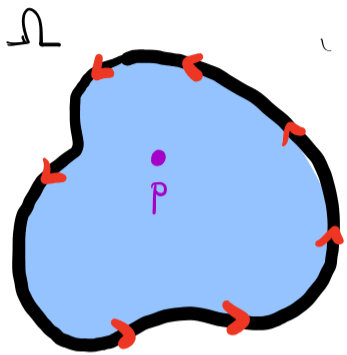
\includegraphics[width=\textwidth]{LECTURE_4/omega.png}.
                \caption{$\Omega$}
            \end{subfigure}
            \hfill
            \begin{subfigure}{0.4\textwidth}
                \centering
                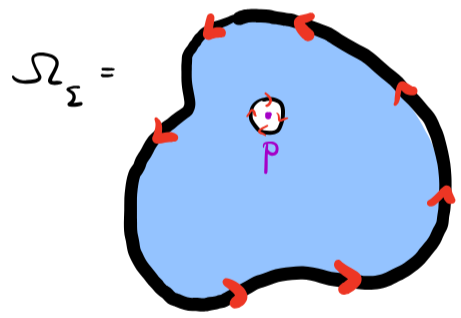
\includegraphics[width=\textwidth]{LECTURE_4/omega-epsilon.png}
                \caption{$\Omega_{\epsilon} = \Omega \setminus D_{\epsilon}(p)$}
            \end{subfigure}
        \end{figure}
        1) Assume $p$ not in $\Omega$ and suppose $f$ is differentiable in $\Omega$ such that:
        $$f = \frac{1}{z - p}$$
        And $\partial \Omega$ is a simple closed curve. So by Green's Theorem:
        \begin{align*}
            \frac{\partial f}{\partial x} & = \frac{\partial}{\partial x} \frac{1}{z - p} = -\frac{1}{(z - p)^2} \\
            \frac{\partial f}{\partial y} & = \frac{\partial}{\partial y} \frac{1}{z - p} =- \frac{i}{(z - p)^2} \\
        \end{align*}
        Then by the Cauchy-Riemann equations:
        $$ \frac{\partial f}{\partial x} - i\frac{\partial f}{\partial y} = 0 $$
        So by Green's Theorem:
        $$ \int_{\partial \Omega} f dz = 0 $$

        2) Assume $p \in \Omega$. Green's theorem doesn't apply here, so we need to be a bit more clever.\\
        Let $D_{\epsilon}(p)$ be the disk of radius $\epsilon$ centered at $p$, essentially, we want to remove the point stopping us from applying Green's Theorem. And we make $\epsilon$ small. So by Green's Theorem:
        \begin{align*}
            0 = \int_{\partial \Omega_\epsilon} f dz & = \int_{\partial \Omega} f dz - \int_{\partial D_{\epsilon}(p)} f dz \\
        \end{align*}
        Where $\partial D_{\epsilon}(p) = \partial \{|z-p| \leq \epsilon\}$ is equal to
        \begin{figure}[H]
            \centering
            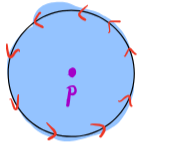
\includegraphics[width=0.5\textwidth]{LECTURE_4/epsilon.png}
            \caption{Epsilon Disk}
        \end{figure}

        \begin{align*} \int_{\partial \Omega_{\epsilon}} \frac{dz}{z - p}                                         & = 0                                                                    \\
               \int_{\partial \Omega} \frac{dz}{z - p} - \int_{\partial D_{\epsilon}(p)} \frac{dz}{z - p} & = 0                                                                    \\
               \int_{\partial \Omega} \frac{dz}{z - p}                                                    & = \int_{\partial D_{\epsilon}(p)} \frac{dz}{z - p}                     \\
               \rightarrow \partial D_{\epsilon}                                                          & = p + \epsilon e^{it} \quad 0 \leq t \leq 2\pi                         \\
               \int_{\partial D_{\epsilon}(p)} \frac{dz}{z - p}                                           & = \int_{0}^{2\pi} \frac{i\epsilon e^{it}}{\epsilon e^{it}} dt = 2\pi i \\
               \int_{\partial \Omega} \frac{dz}{z - p}                                                    & = 2\pi i
        \end{align*}
    \end{proof}

\end{example}


\begin{theorem}
    [Complex Partial Derivatives]
    The previous example gives us the following theorem:
    Let $f = u + iv$ be differentiable in $\Omega$. Then $f$ is infinitely differentiable in $\Omega$ and the partial derivatives of $f$ are given by:
    \begin{align*}
        \frac{\partial f}{\partial x} & = \frac{\partial u}{\partial x} + i\frac{\partial v}{\partial x} \\
        \frac{\partial f}{\partial y} & = \frac{\partial u}{\partial y} + i\frac{\partial v}{\partial y} \\
    \end{align*}
\end{theorem}